\documentclass[letterpaper,10pt,conference]{ieeeconf}

\IEEEoverridecommandlockouts
\overrideIEEEmargins

\usepackage{graphicx}
\usepackage{booktabs}
\usepackage{amsmath}
\usepackage{amssymb}
\usepackage{array}
\usepackage{microtype}
\usepackage{algorithm}
\usepackage{algorithmic}
\usepackage{cite}
\usepackage{url}
\usepackage[colorlinks=true,linkcolor=blue,citecolor=blue,urlcolor=blue,breaklinks=true]{hyperref}
\urlstyle{same}


\title{\LARGE \bf AMD-Agent: Autonomous Malware Detection Agent}

\author{
\IEEEauthorblockN{Baruh Ifraimov\textsuperscript{1} and Dor Cohen\textsuperscript{1}}
\IEEEauthorblockA{Department of Cyber Security\\
Ariel University Center of Samaria, Ariel, Israel}
}
\begin{document}

\maketitle
\thispagestyle{empty}
\pagestyle{empty}

\begin{abstract}
This project presents AMD-Agent, an autonomous LLM-assisted continual-learning system for PE malware detection. The agent collects malware and benign samples from live sources, validates downloaded binaries, extracts static PE features, monitors concept drift, and retrains a LightGBM classifier using replay-based learning. A local Ollama-based LLM agent supports the workflow by assisting with source selection, CTI filtering, PE error triage, and drift explanations, while deterministic fallbacks keep the system operational when the LLM is unavailable. To evaluate updates reliably, AMD-Agent compares the previous and updated models on a strict temporal holdout excluded from training, reporting Accuracy, Precision, Recall, and False Positive Rate (FPR). The result is an adaptive malware detection pipeline that combines autonomous collection, LLM-assisted decision making, continual retraining, and measurable before/after evaluation.
Our implementation and source code are available on GitHub \cite{amdagentgithub}.
\end{abstract}

\section{Introduction}

Malware detection is a continuously changing problem. New malware variants, packers, and evasion techniques appear over time, while benign software also changes through new versions and build processes. A classifier trained once on a fixed dataset may therefore become outdated when deployed in a live environment. This motivates the need for continual learning and reliable update evaluation.

AMD-Agent addresses this problem by implementing an autonomous pipeline for PE malware detection without relying on predefined datasets. The system discovers malware and benign samples from external sources, downloads and validates PE files, extracts static features, monitors drift, performs inference, and retrains the model when new labeled data or drift evidence is available. The classifier is based on LightGBM with feature selection and FPR-aware threshold calibration.

A key part of the project is avoiding misleading evaluation. For each model update, AMD-Agent creates a strict chronological holdout and excludes it from retraining. The previous and updated models are then evaluated on the same holdout using Accuracy, Precision, Recall, and FPR. This enables a direct before/after comparison while reducing data leakage.

The system also includes optional local LLM support through Ollama for source selection, CTI filtering, and drift explanations. The LLM is not the malware classifier; it assists the agent’s workflow while deterministic fallbacks keep the system operational. Overall, AMD-Agent demonstrates a practical approach for adaptive malware detection with automated collection, retraining, and evaluation.

\section{Related Work}

This section reviews the fundamental literature and tooling that influenced the architecture of AMD-Agent. A consolidated critical analysis of their methodologies, limitations, and direct contributions to our system design is provided in Table \ref{tab:related_work}.

\textbf{Data Acquisition and Parsing:} To facilitate an autonomous pipeline without predefined datasets, we utilize the \textbf{MalwareBazaar API}~\cite{malwarebazaar} as our primary live malware source. While it provides metadata-rich, real-world samples, it requires strict sandboxing to mitigate execution risks. To safely process these incoming streams, we rely on \textbf{\textit{pefile}}~\cite{pefile}, a mature Python library for static Windows Portable Executable (PE) parsing. Although limited by its inability to observe runtime behavior, its safe API perfectly aligns with our lightweight feature extraction stage.

\textbf{Feature Representation and Continual Learning:} Our structural feature vector is directly inspired by \textbf{EMBER}~\cite{anderson2018ember}, which establishes a strong baseline for static malware classification, despite its inherent vulnerability to advanced packing techniques. Because these static distributions shift over time, we employ \textbf{River}'s \textbf{ADWIN} algorithm~\cite{riveradwin} for lightweight, online drift detection based on section entropy. Once drift is identified, we address catastrophic forgetting by adopting the diversity-aware replay methodology proposed in \textbf{MADAR}~\cite{rahman2025madar}, mixing historical samples with new data during \textbf{LightGBM} retraining. \textbf{Optuna}~\cite{akiba2019optuna} is integrated into this retraining phase to automate hyperparameter optimization via tree-structured parzen estimators, ensuring that the updated LightGBM model configuration adapts efficiently to the shifted feature space without manual tuning.

\textbf{Evaluation Methodology:} Finally, to evaluate our model updates reliably, we adopted the \textbf{TESSERACT}~\cite{pendlebury2019tesseract} evaluation framework. Random train-test splits often overestimate malware classification performance due to temporal data leakage. By enforcing strict chronological splits, \textbf{TESSERACT} ensures a realistic before/after comparison, even though it occasionally requires skipping evaluation phases when temporal windows yield single-class holdouts.

\begin{table*}[htbp]
\centering
\caption{Summary of Papers and Tools Used in AMD-Agent}
\label{tab:related_work}
\scriptsize
\renewcommand{\arraystretch}{1.25}
\begin{tabular}{|>{\raggedright\arraybackslash}p{1.9cm}|>{\raggedright\arraybackslash}p{1.7cm}|>{\raggedright\arraybackslash}p{3.0cm}|>{\raggedright\arraybackslash}p{3.4cm}|>{\raggedright\arraybackslash}p{4.6cm}|}
\hline
\textbf{Item} & \textbf{Type} & \textbf{Purpose} & \textbf{Pros / Cons} & \textbf{How We Used It} \\
\hline

TESSERACT~\cite{pendlebury2019tesseract} & Paper / Evaluation &
Chronological malware evaluation. &
Pros: reduces temporal leakage. Cons: can skip when splits are single-class. &
Used for time-aware Accuracy, Precision, Recall, and FPR evaluation, including before/after model-update comparison. \\
\hline

EMBER~\cite{anderson2018ember} & Paper / Method &
Static PE malware feature representation. &
Pros: strong malware ML baseline. Cons: static features can be evaded by packing. &
Inspired our 2304-dimensional EMBER-like static feature vector. \\
\hline

MADAR~\cite{rahman2025madar} & Paper / Method &
Replay-based continual learning. &
Pros: reduces catastrophic forgetting. Cons: depends on stored historical samples. &
Guided family-aware replay selection before retraining with new drifted samples. \\
\hline

LangGraph~\cite{langgraph} & Tool &
Agent workflow orchestration. &
Pros: modular routing and state passing. Cons: requires careful state cleanup. &
Built the graph nodes for source selection, fetch, validation, feature extraction, drift detection, retraining, inference, and evaluation. \\
\hline

pefile~\cite{pefile} & Tool &
Static parsing of Windows PE files. &
Pros: mature and safe. Cons: static-only, no runtime behavior. &
Extracted PE headers, sections, directories, imports, exports, entropy, and parser warnings. \\
\hline

Ollama~\cite{ollama} & Tool &
Local LLM semantic sidecar. &
Pros: local semantic analysis. Cons: best-effort output, requires fallback logic. &
Used for source strategy support, CTI hash verdicts, PE parse-error triage, optional source-page refinement, and drift explanations. \\
\hline

Optuna~\cite{akiba2019optuna} & Tool &
Automated hyperparameter optimization. &
Pros: efficient Bayesian search (TPE), time-capped trials. Cons: high search overhead if unconstrained. &
Ran up to 25 time-capped trials on the 384-feature validation slice to optimize LightGBM hyperparameters under strict FPR constraints. \\
\hline

MalwareBazaar~\cite{malwarebazaar} & Tool / API &
Live malware hash and sample source. &
Pros: real-world malware and metadata. Cons: quotas, noisy samples, availability limits. &
Used for malware discovery, PE hash verification, and controlled sample download. \\
\hline

OTX~\cite{otx} & Tool / API &
Live CTI pulse source. &
Pros: fresh threat intelligence. Cons: noisy and unstructured text. &
Extracted SHA256 indicators from pulses, filtered context with Ollama, then validated hashes before queueing. \\
\hline

River / ADWIN~\cite{riveradwin} & Tool / Algorithm &
Streaming concept drift detection. &
Pros: online and lightweight. Cons: threshold tuning is required. &
Monitored entropy shifts and helped trigger retraining when drift appeared. \\
\hline

\end{tabular}
\end{table*}

\section{System Architecture and Agent Design}
AMD-Agent operates as a graph-based controller managed by a LangGraph state machine. Rather than executing as a single monolithic script, the system can run as a persistent loop traversing distinct collection, ML, and evaluation forks.

\subsection{State Management}

The system separates short-term runtime data from long-term stored data. This keeps each pipeline run simple while still allowing the agent to continue learning over time.

\begin{enumerate}
    \item \textbf{Current Run State (\texttt{AgentState}):}
    Each pipeline run begins with a newly initialized \texttt{AgentState}. This object retains only the data required for the active batch, including discovered hashes, downloaded file paths, extracted feature vectors, predictions, and routing flags (e.g., \texttt{drift\_detected}). To guarantee isolation, the source selector clears these fields before each run so legacy data cannot affect the new batch.

    \item \textbf{LangGraph Execution State:}
    LangGraph uses this state while moving between nodes such as source selection, download, validation, feature extraction, drift monitoring, inference, retraining, and evaluation. The \texttt{MemorySaver} checkpointer helps LangGraph manage the state during execution, but it is not treated as the system's permanent memory.

    \item \textbf{Persistent Storage:}
    Long-term information is stored outside the graph state. SQLite stores the sample database, including hashes, file paths, labels, extracted features, predictions, sample status, and ingestion time. Corrupted samples are marked in the database so they are not repeatedly processed. The trained LightGBM model is saved with Joblib as \texttt{model.pkl}, and the ADWIN drift detector state is saved as \texttt{adwin.joblib}. Evaluation, drift, and model update records are written to log files under \texttt{data/}.
\end{enumerate}

\subsection{Dynamic Feedback Control Loop}
The architecture relies on a closed-loop feedback mechanism governed by three main routing decisions (Algorithm \ref{alg:core_loop}):
\begin{itemize}
    \item \textbf{Fork A (Collection):} Evaluates SQLite class distributions and provider yield metrics recorded in SQLite. If the system lacks specific classes, it routes to discovery modules targeting those deficits (e.g., Sysinternals for benign files). Sources are ranked by recent success rate, low-yield providers can be cooled down, and collection/fetch/validation/update steps use reusable tools.

    \item \textbf{Fork B (Machine Learning):} Evaluates the current batch against the ADWIN monitor. If drift is flagged, the graph routes dynamically to the continual learning (MADAR) nodes; otherwise, it passes directly to the inference node.
    
    \item \textbf{Fork C (Evaluation Gate):} Triggers chronological TESSERACT evaluations periodically every $N$ steady runs and after drift or retraining. After each successful model update, the previous and updated models are compared on the same strict temporal holdout, and the delta is written to \texttt{model\_update\_log.jsonl}.

\end{itemize}

\begin{algorithm}[htbp]
\caption{AMD-Agent Core Control Loop}
\label{alg:core_loop}
\small
\begin{algorithmic}[1]
\REQUIRE SQLite DB $\mathcal{C}$, Classifier $\mathcal{M}$, ADWIN $\mathcal{A}$
\LOOP
    \STATE $L \gets \text{BalanceController}(\mathcal{C}.\text{counts})$ \COMMENT{Determine needed class}
    \STATE $B_{\text{batch}} \gets \text{DownloadAndValidate}(L)$
    \FOR{each file $f \in B_{\text{batch}}$}
        \STATE $\mathbf{x}_f \gets \text{ExtractFeatures}(f)$
        \STATE $\mathcal{C}.\text{Insert}(f, \mathbf{x}_f)$
    \ENDFOR
    
    \IF{$\text{Drift}(\mathcal{A}, \mathbf{x}_{B}, \text{Entropy}_{B})$}
        \STATE Trigger $\leftarrow$ \textbf{Drift}
    \ELSIF{$\mathcal{C}.\text{UntrainedCount} \geq 50$}
        \STATE Trigger $\leftarrow$ \textbf{Threshold}
    \ELSE
        \STATE Trigger $\leftarrow$ \textbf{None}
    \ENDIF
    
    \IF{Trigger $\in \{\text{Drift, Threshold}\}$}
        \STATE $\mathcal{M} \gets \text{MadarRetrain}(\mathcal{C}, B_{\text{batch}})$
    \ELSE
        \FOR{each file $f \in B_{\text{batch}}$}
            \STATE $\mathcal{C}_f.\text{prediction} \gets \text{Predict}(\mathcal{M}, \mathbf{x}_f)$
        \ENDFOR
    \ENDIF
    
    \IF{EvalDue \OR Trigger $\neq$ None}
        \STATE \text{LogTesseractEval}($\mathcal{C}, \mathcal{M}$)
    \ENDIF
\ENDLOOP
\end{algorithmic}
\end{algorithm}

\subsection{LLM Sidecar Intelligence (Ollama)}
Ollama is used as a local semantic sidecar, not as the malware classifier and not as a safety gate. It supports the agent in several roles: source strategy selection with reusable CTI tools, structured filtering of unstructured CTI text from OTX and curated feeds into SHA256 malware verdicts, PE parse-error triage during feature extraction, optional PE source page refinement, and explanation of concept-drift events from drift statistics and anomalous PE features.

All LLM outputs are best-effort and have deterministic fallbacks. Candidate samples still pass through hard validation gates: MalwareBazaar PE verification, \texttt{MZ} and \texttt{PE\textbackslash0\textbackslash0} signature checks, SHA256 filename verification, duplicate detection, and SQLite quarantine for corrupted samples. This design provides LLM-based content analysis, autonomous source reasoning, and drift explainability without making pipeline correctness depend on the LLM.


\section{Methodology}

\subsection{Safe Malware Acquisition and Sandboxing}
Because the system continuously ingests live, weaponized PE files, the pipeline enforces strict isolation controls. It runs within a dedicated Docker bridge network (\texttt{malware\_net}), while \texttt{iptables} egress rules block outbound traffic to private subnets, preserving required DNS, Ollama, and public access.

Crucially, \textbf{downloaded binaries are never executed}. Files are written directly to a sandbox directory with restrictive \texttt{0600} permissions. Before progressing to feature extraction, deterministic validation gates verify the DOS \texttt{MZ} header, the \texttt{PE\textbackslash0\textbackslash0} signature at \texttt{e\_lfanew}, the SHA256 filename/content match, and duplicate status. Files failing these checks are logged to SQLite as \texttt{corrupted} and permanently quarantined to prevent cyclical re-fetching.

\subsection{Static Feature Representation}
Static analysis projects each validated binary into a fixed-size feature space without requiring execution. Each file maps to a uniform vector:
\begin{equation}
    \mathbf{x} = (f_1, f_2, \ldots, f_{2304}) \in \mathbb{R}^{2304}
\end{equation}
This 2304-dimensional EMBER-like representation combines PE headers and directories, section metadata, import/export information, printable string statistics, byte histograms, byte-entropy histograms, Authenticode and overlay indicators, and lightweight instruction-level features:
\begin{itemize}
    \item \textbf{Entropy and Packing Signals:} Section entropy and byte-window entropy variations, which are sensitive to packing, encryption, and obfuscation, are calculated as:
    \begin{equation}
        H(X) = -\sum_{b=0}^{255} p(b)\,\log_2 p(b)
    \end{equation}
    where $p(b)$ is the byte frequency.
    \item \textbf{PE Structure and Behavioral Surface:} The extractor records structural and behavioral static signals such as section permissions, suspicious section names, imported APIs, exported symbols, URLs, filesystem paths, registry strings, executable-memory APIs, and lightweight instruction-level patterns. This preserves a fully static pipeline while capturing indicators related to packing, persistence, API usage, and code behavior.
\end{itemize}

\subsection{Classifier and Dynamic Threshold Calibration}
To optimize classification speed, an XGBoost-based feature ranking step evaluates the $\mathbb{R}^{2304}$ matrix and isolates the top 384 dimensions by feature importance. A LightGBM binary classifier is then trained exclusively on this subset. 

In cybersecurity operations, False Positive Rate (FPR) containment is paramount. After hyperparameter tuning via Optuna (a Python library for automatic hyperparameter search), the classification threshold $\tau$ is dynamically calibrated on the validation split. The target FPR becomes strictly tighter as the number of trainable benign samples ($N_0$) in the corpus grows:
\begin{equation}
\text{target\_fpr}(N_0) =
\begin{cases}
0.05 & N_0 < 1000 \\
0.01 & 1000 \le N_0 < 5000 \\
0.001 & N_0 \ge 5000
\end{cases}
\end{equation}
The FPR target starts relaxed during bootstrap, then tightens automatically to ($\leq 0.1\%$) once the benign corpus is large enough for steady-state operation.

\subsection{Drift Detection}

The agent checks for concept drift (when malware patterns change) using two methods. If either check triggers, the graph routes the current pass to explanation and retraining instead of normal inference.

\textbf{Entropy stream (ADWIN).} 
For each validated file, the system computes the average PE section entropy and streams it into River's ADWIN detector, which raises an alert if the entropy distribution suddenly shifts.

\textbf{Feature stream (sliding windows).} 
The system also tracks its top $d=64$ features. It compares the most recent $W=20$ samples (the current window) against the 20 samples right before them (the previous window). It looks for two types of changes:

1. \textbf{Mean shift:} Did the average values of the features move? 
\begin{equation}
    \mathrm{mean\_shift} = \frac{1}{d}\sum_{j=1}^{d}\frac{\bigl|\mu^{\mathrm{curr}}_j-\mu^{\mathrm{prev}}_j\bigr|}{\sigma^{\mathrm{prev}}_j+\epsilon}
\end{equation}

2. \textbf{Correlation shift:} Do the features still relate to each other in the same way? This checks the relationships between dimensions, not just their individual levels. It calculates the mean absolute difference between the Pearson correlation matrices ($\mathbf{C}^{\mathrm{prev}}$ and $\mathbf{C}^{\mathrm{curr}}$) of the two windows:
\begin{equation}
    \Delta_{\mathrm{corr}} = \mathrm{mean}\bigl(\bigl|\mathbf{C}^{\mathrm{curr}} - \mathbf{C}^{\mathrm{prev}}\bigr|\bigr)
\end{equation}

\textbf{Trigger Conditions.}
The system officially flags a drift if any of these limits are crossed:
\begin{equation}
    \text{drift} \;\Leftrightarrow\; \text{ADWIN}_{\mathrm{alert}} \;\lor\; \mathrm{mean\_shift} \ge 1.5 \;\lor\; \Delta_{\mathrm{corr}} \ge 0.35
\end{equation}

\textbf{Autonomous Mitigation.} 
When drift happens, the agent saves its current performance scores. An LLM can optionally write a plain-text summary explaining what changed. Next, the model retrains itself (the MADAR method). It mixes the new batch of files with up to 3,000 carefully chosen past files so it does not forget older malware. To ensure the new model is tested fairly, the newest 15\% of all data is kept completely hidden during training.

\subsection{Catastrophic Forgetting Mitigation (MADAR Replay)}
To avoid forgetting older malware and benign patterns during retraining, the system uses a MADAR-inspired replay strategy. When drift or a retraining threshold triggers an update, the current drift batch is combined with a bounded replay sample from historical SQLite records, while the strict temporal holdout is excluded from training to keep evaluation clean.

The replay budget is capped at \texttt{REPLAY\_BUDGET = 3000}. Half of the budget is reserved for benign samples selected by uniform random sampling. The remaining half is assigned to malware families using proportional ratio budgeting, so larger observed families receive more replay slots while smaller families are still represented. Inside each malware family, an Isolation Forest ranks samples by anomaly score; the replay set keeps both representative low-anomaly samples and high-anomaly edge cases. This gives the retraining step a compact memory of past decision boundaries while still adapting to newly observed drifted samples.

\section{Experimental Results and Analysis}
The following sections detail the empirical evaluation of the AMD-Agent pipeline, using chronological TESSERACT-style evaluation and model-update logs to reduce temporal leakage.

\subsection{Temporal Performance Decay Analysis}
\begin{figure}[htbp]
\centering
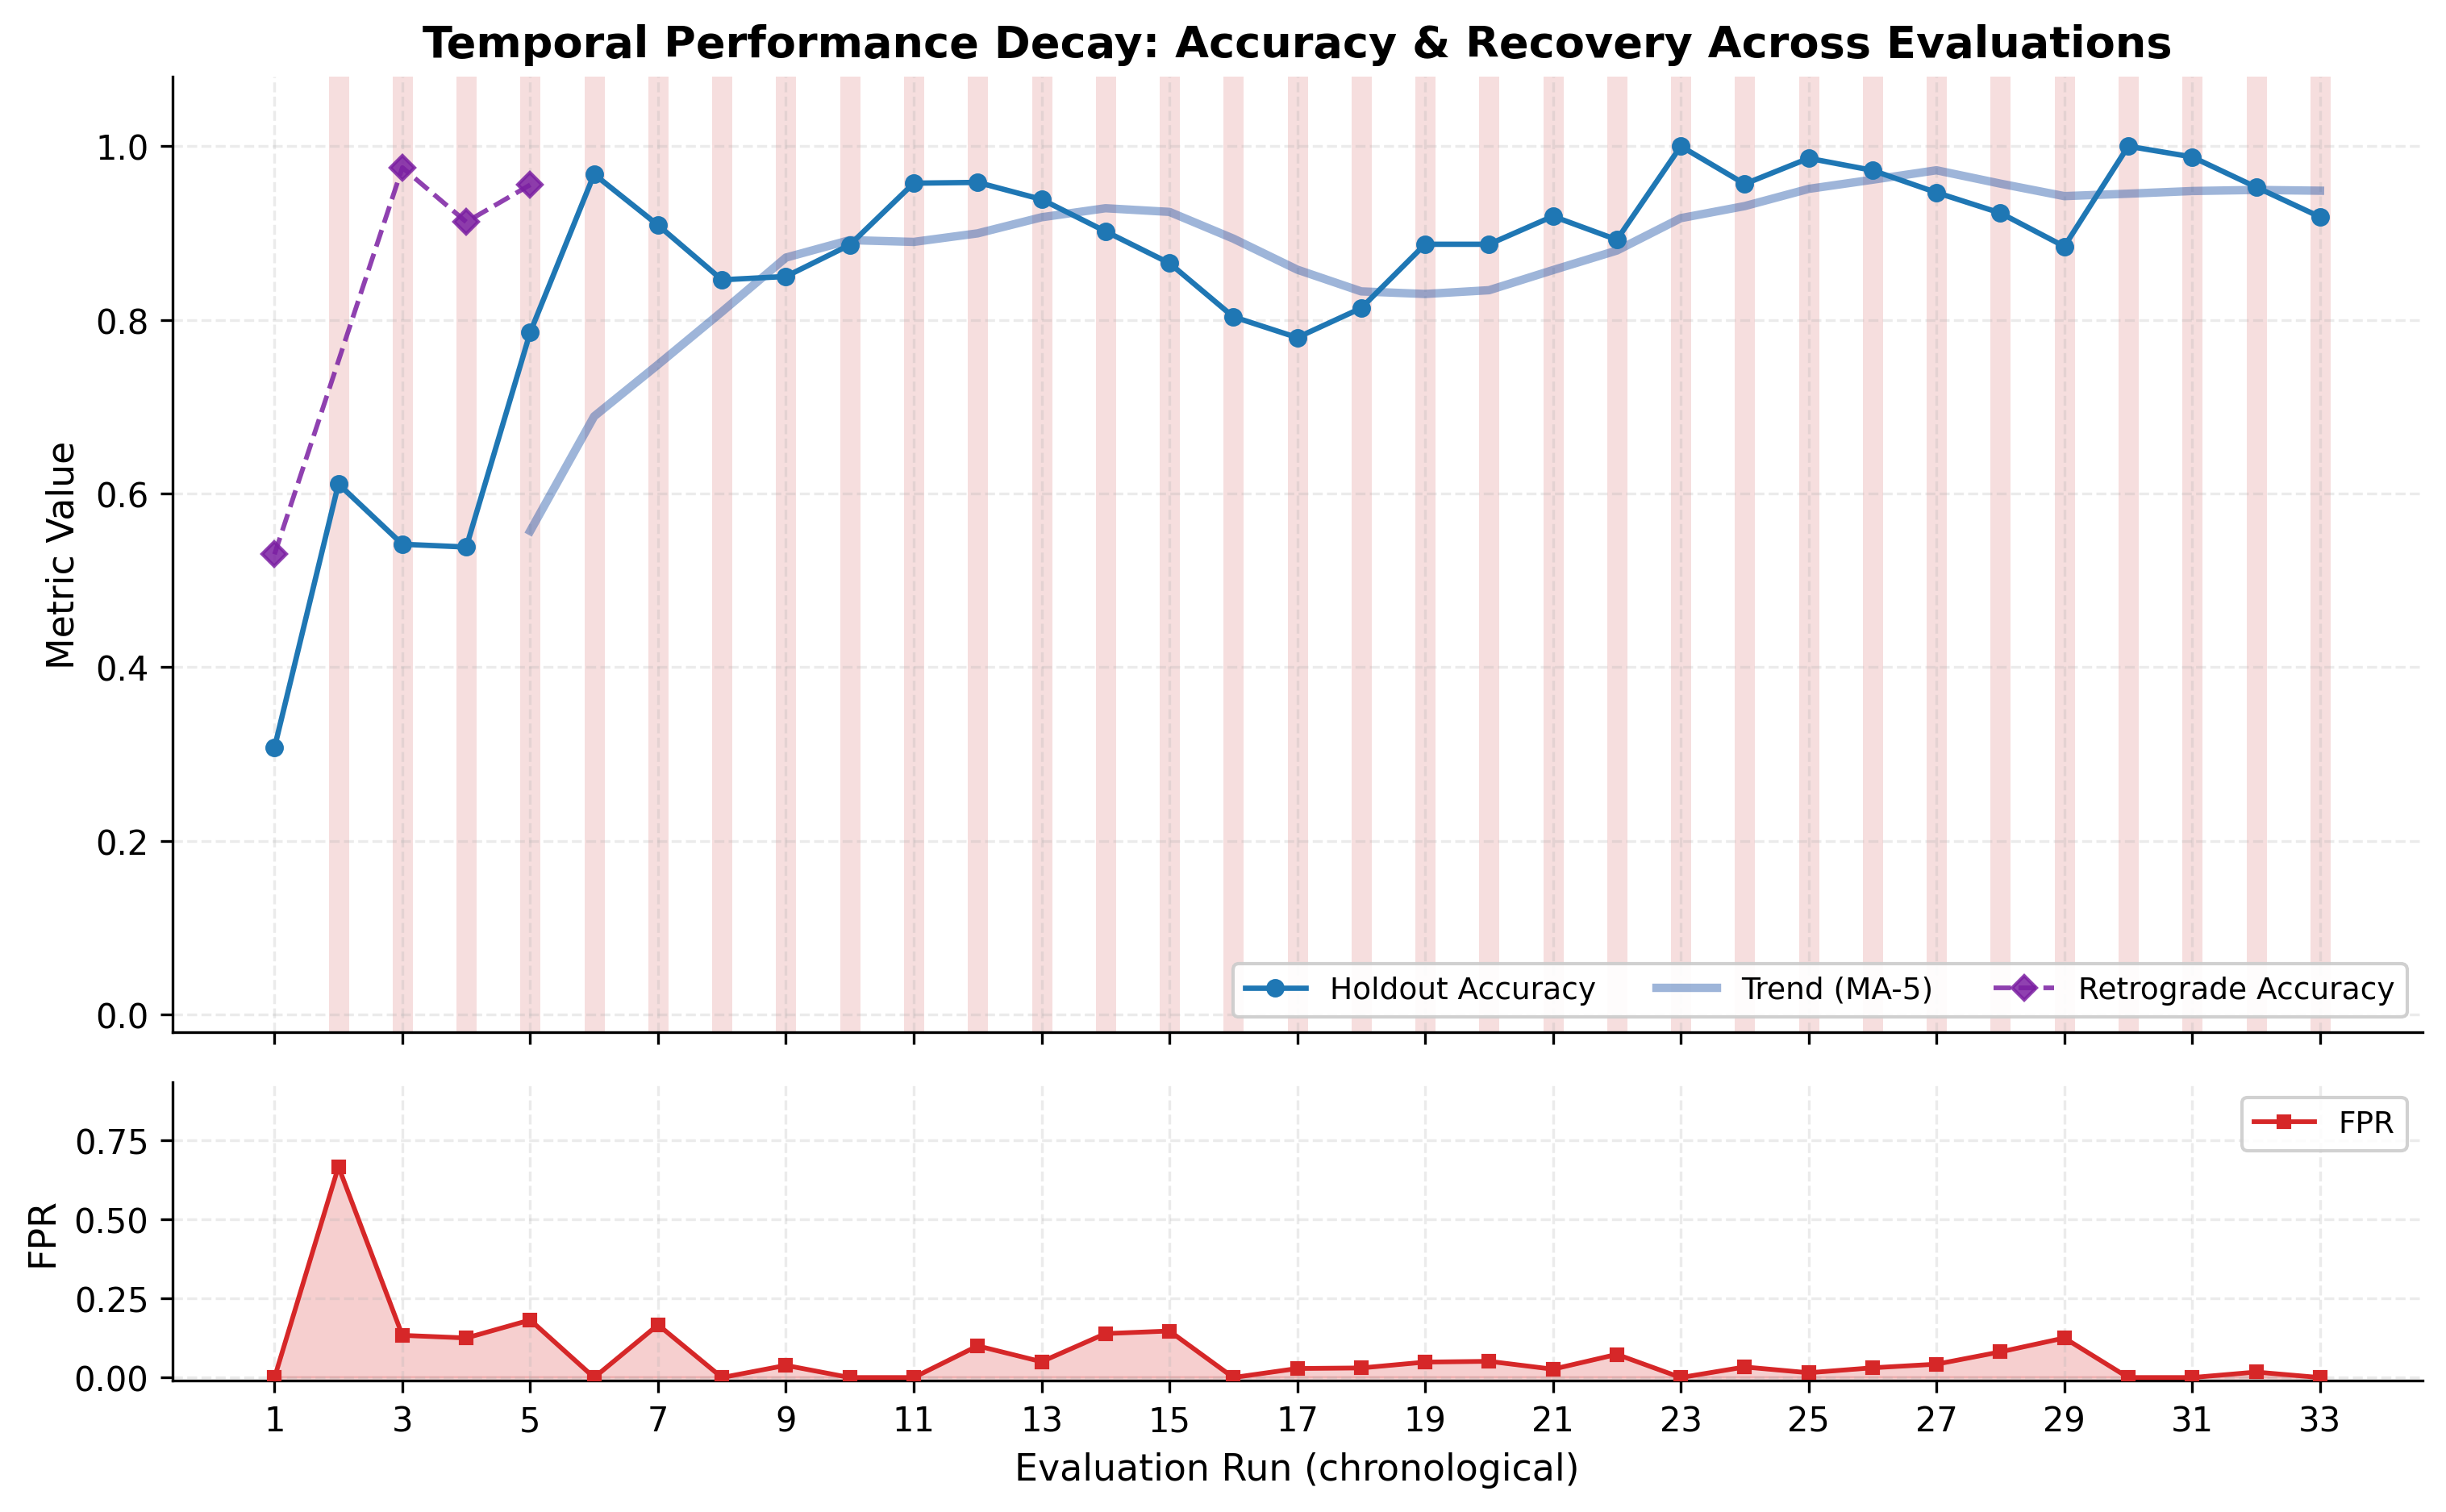
\includegraphics[width=\columnwidth]{figures/temporal_performance_decay.png}
\caption{Accuracy \& Recovery Across Evaluation}
\label{fig:temporal_decay}
\end{figure}

The chronological evaluation shows the expected early instability of a live-learning system, followed by recovery as additional batches are collected and retraining cycles accumulate. Holdout accuracy rises from weak early runs to mostly high steady-state values, while FPR becomes substantially lower after the initial spikes. The moving trend and retrograde checks show that the agent is not only fitting the newest batch, but also preserving useful historical behavior across later evaluation windows.

\subsection{Error and Threshold Analysis}
\IfFileExists{figures/perf_over_time.png}{%
\begin{figure}[htbp]
\centering
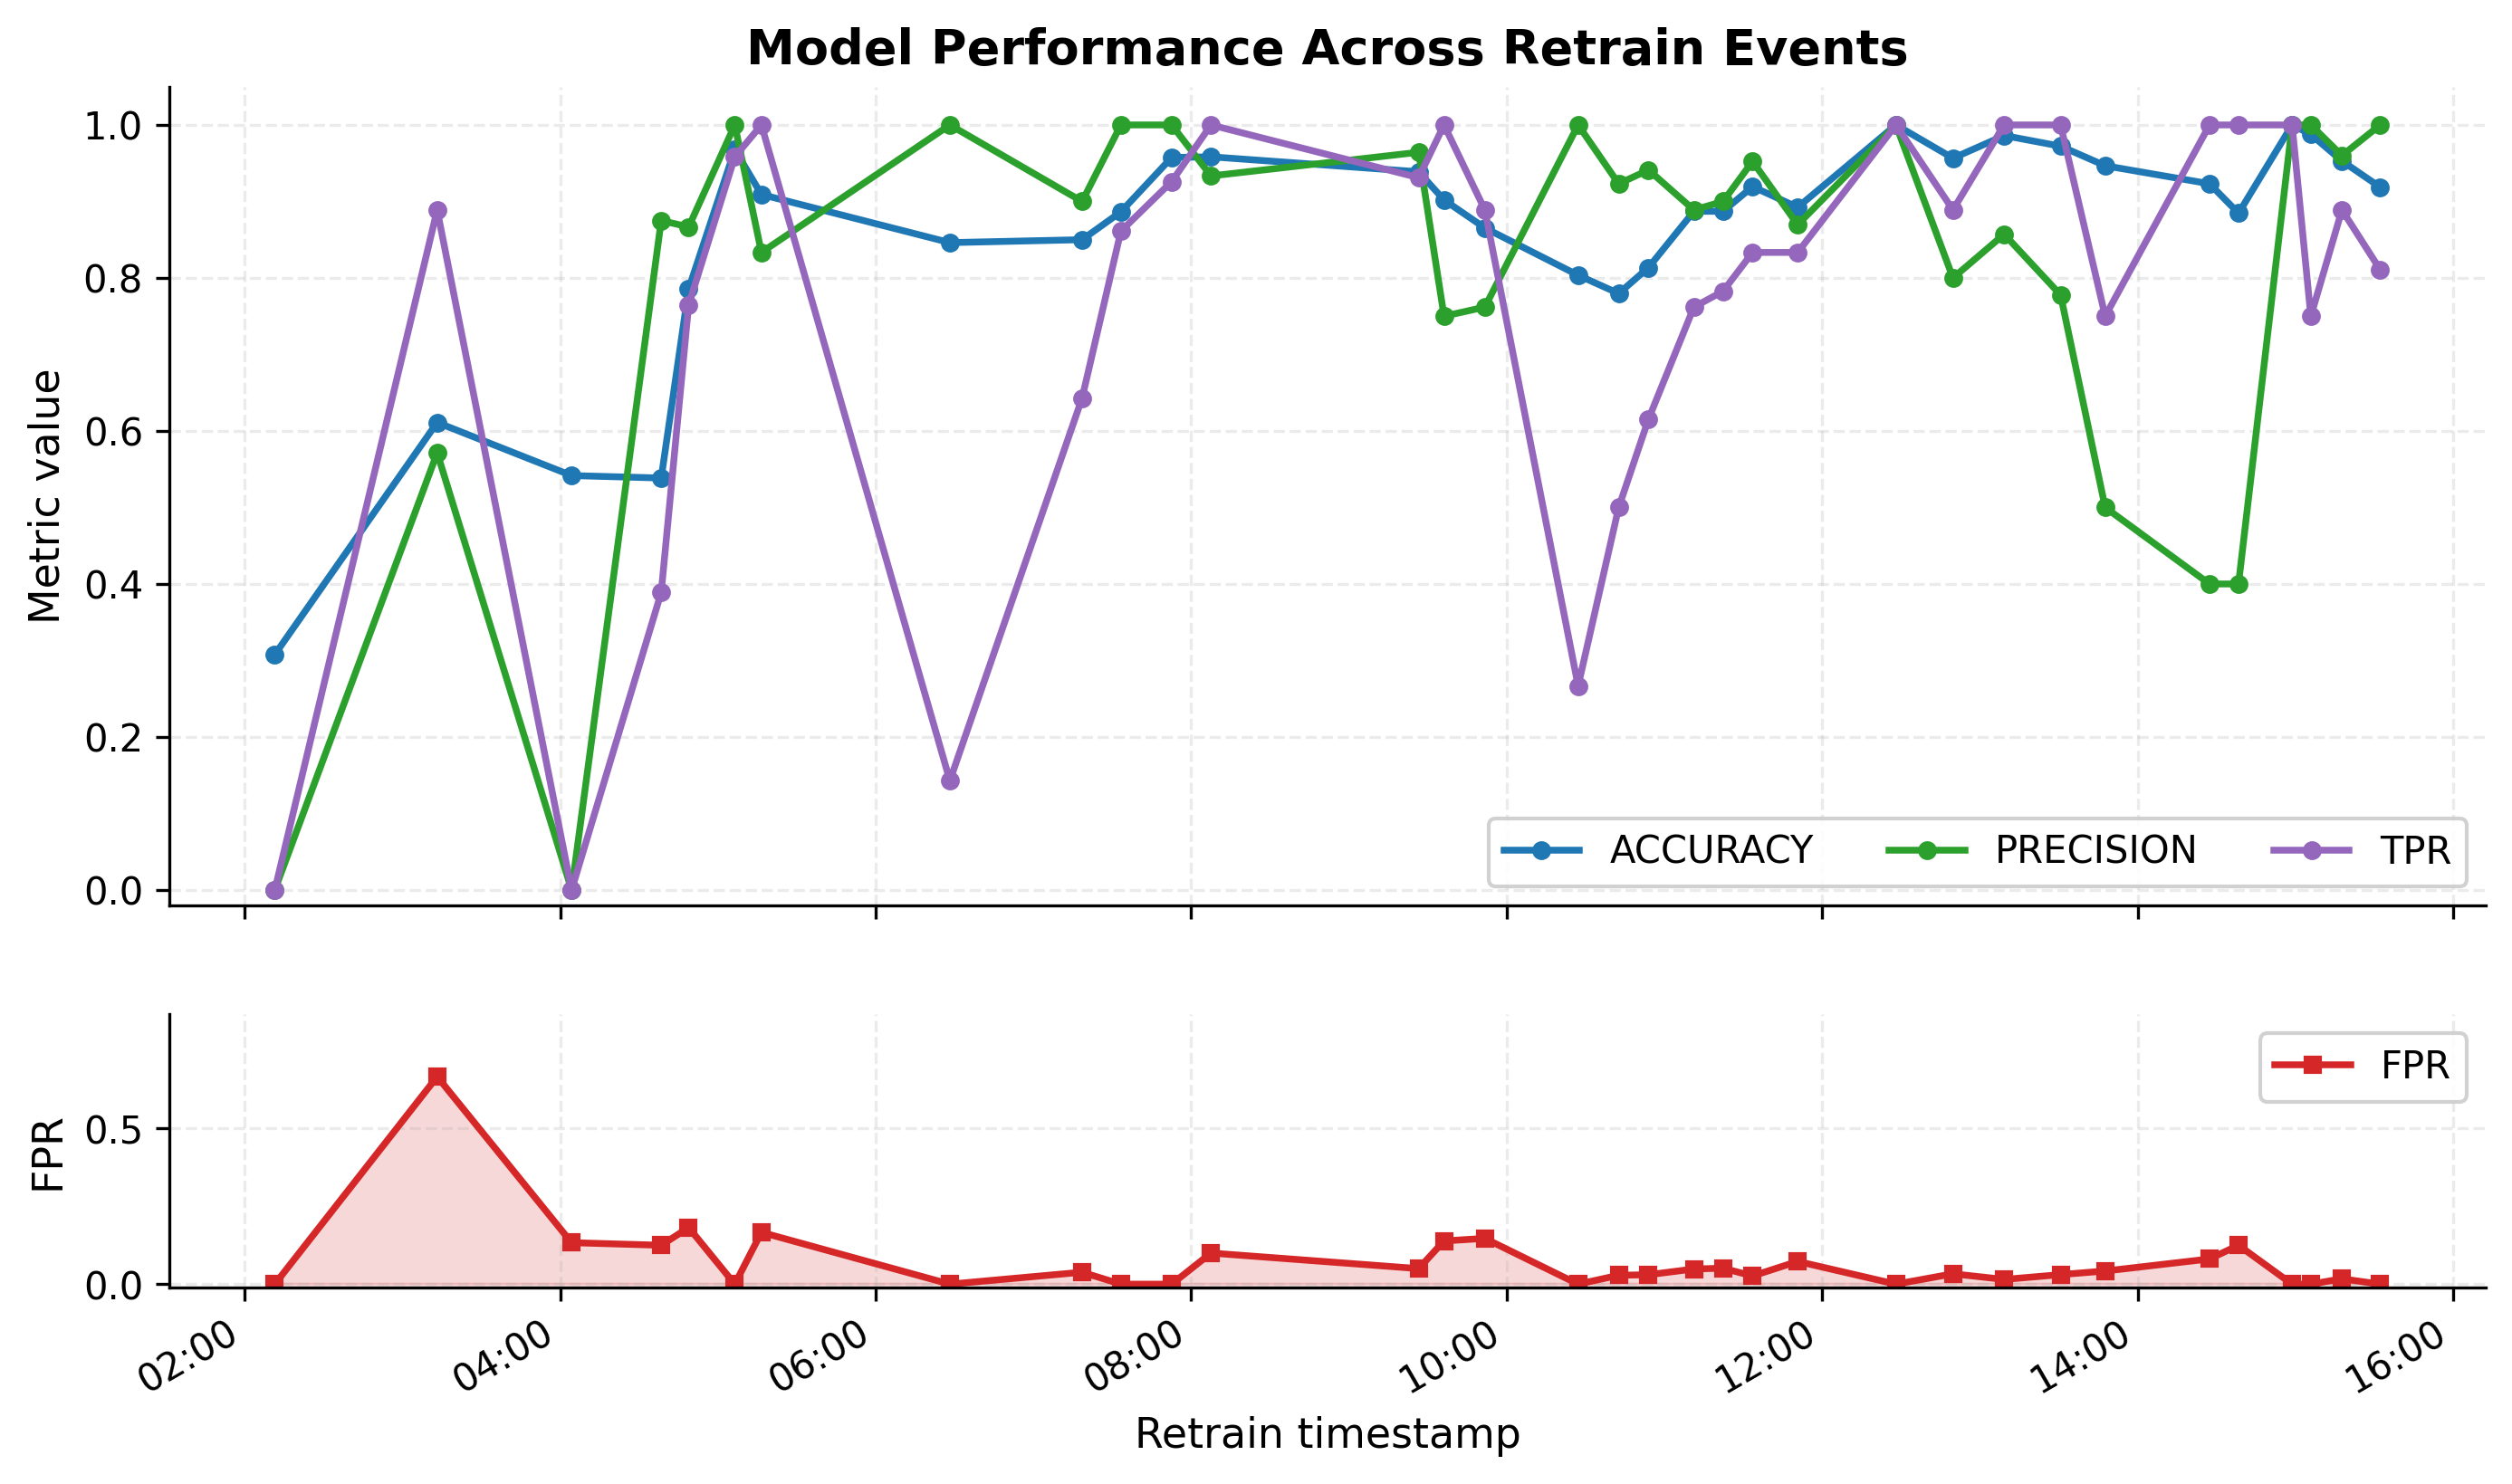
\includegraphics[width=\columnwidth]{figures/perf_over_time.png}
\caption{Accuracy, precision, TPR, and FPR across retrain events.}
\end{figure}
}{}
The model is calibrated around operational FPR control rather than accuracy alone. The results show that early runs can produce unstable FPR, but later retraining generally keeps FPR low while accuracy, precision, and TPR remain high. False negatives may occur when packed or obfuscated samples hide static indicators, so the system records retraining deltas and threshold behavior instead of assuming one fixed model remains reliable over time.

\subsection{Data Provenance and Source Reliability}
\IfFileExists{figures/data_per_source.png}{%
\begin{figure}[htbp]
\centering
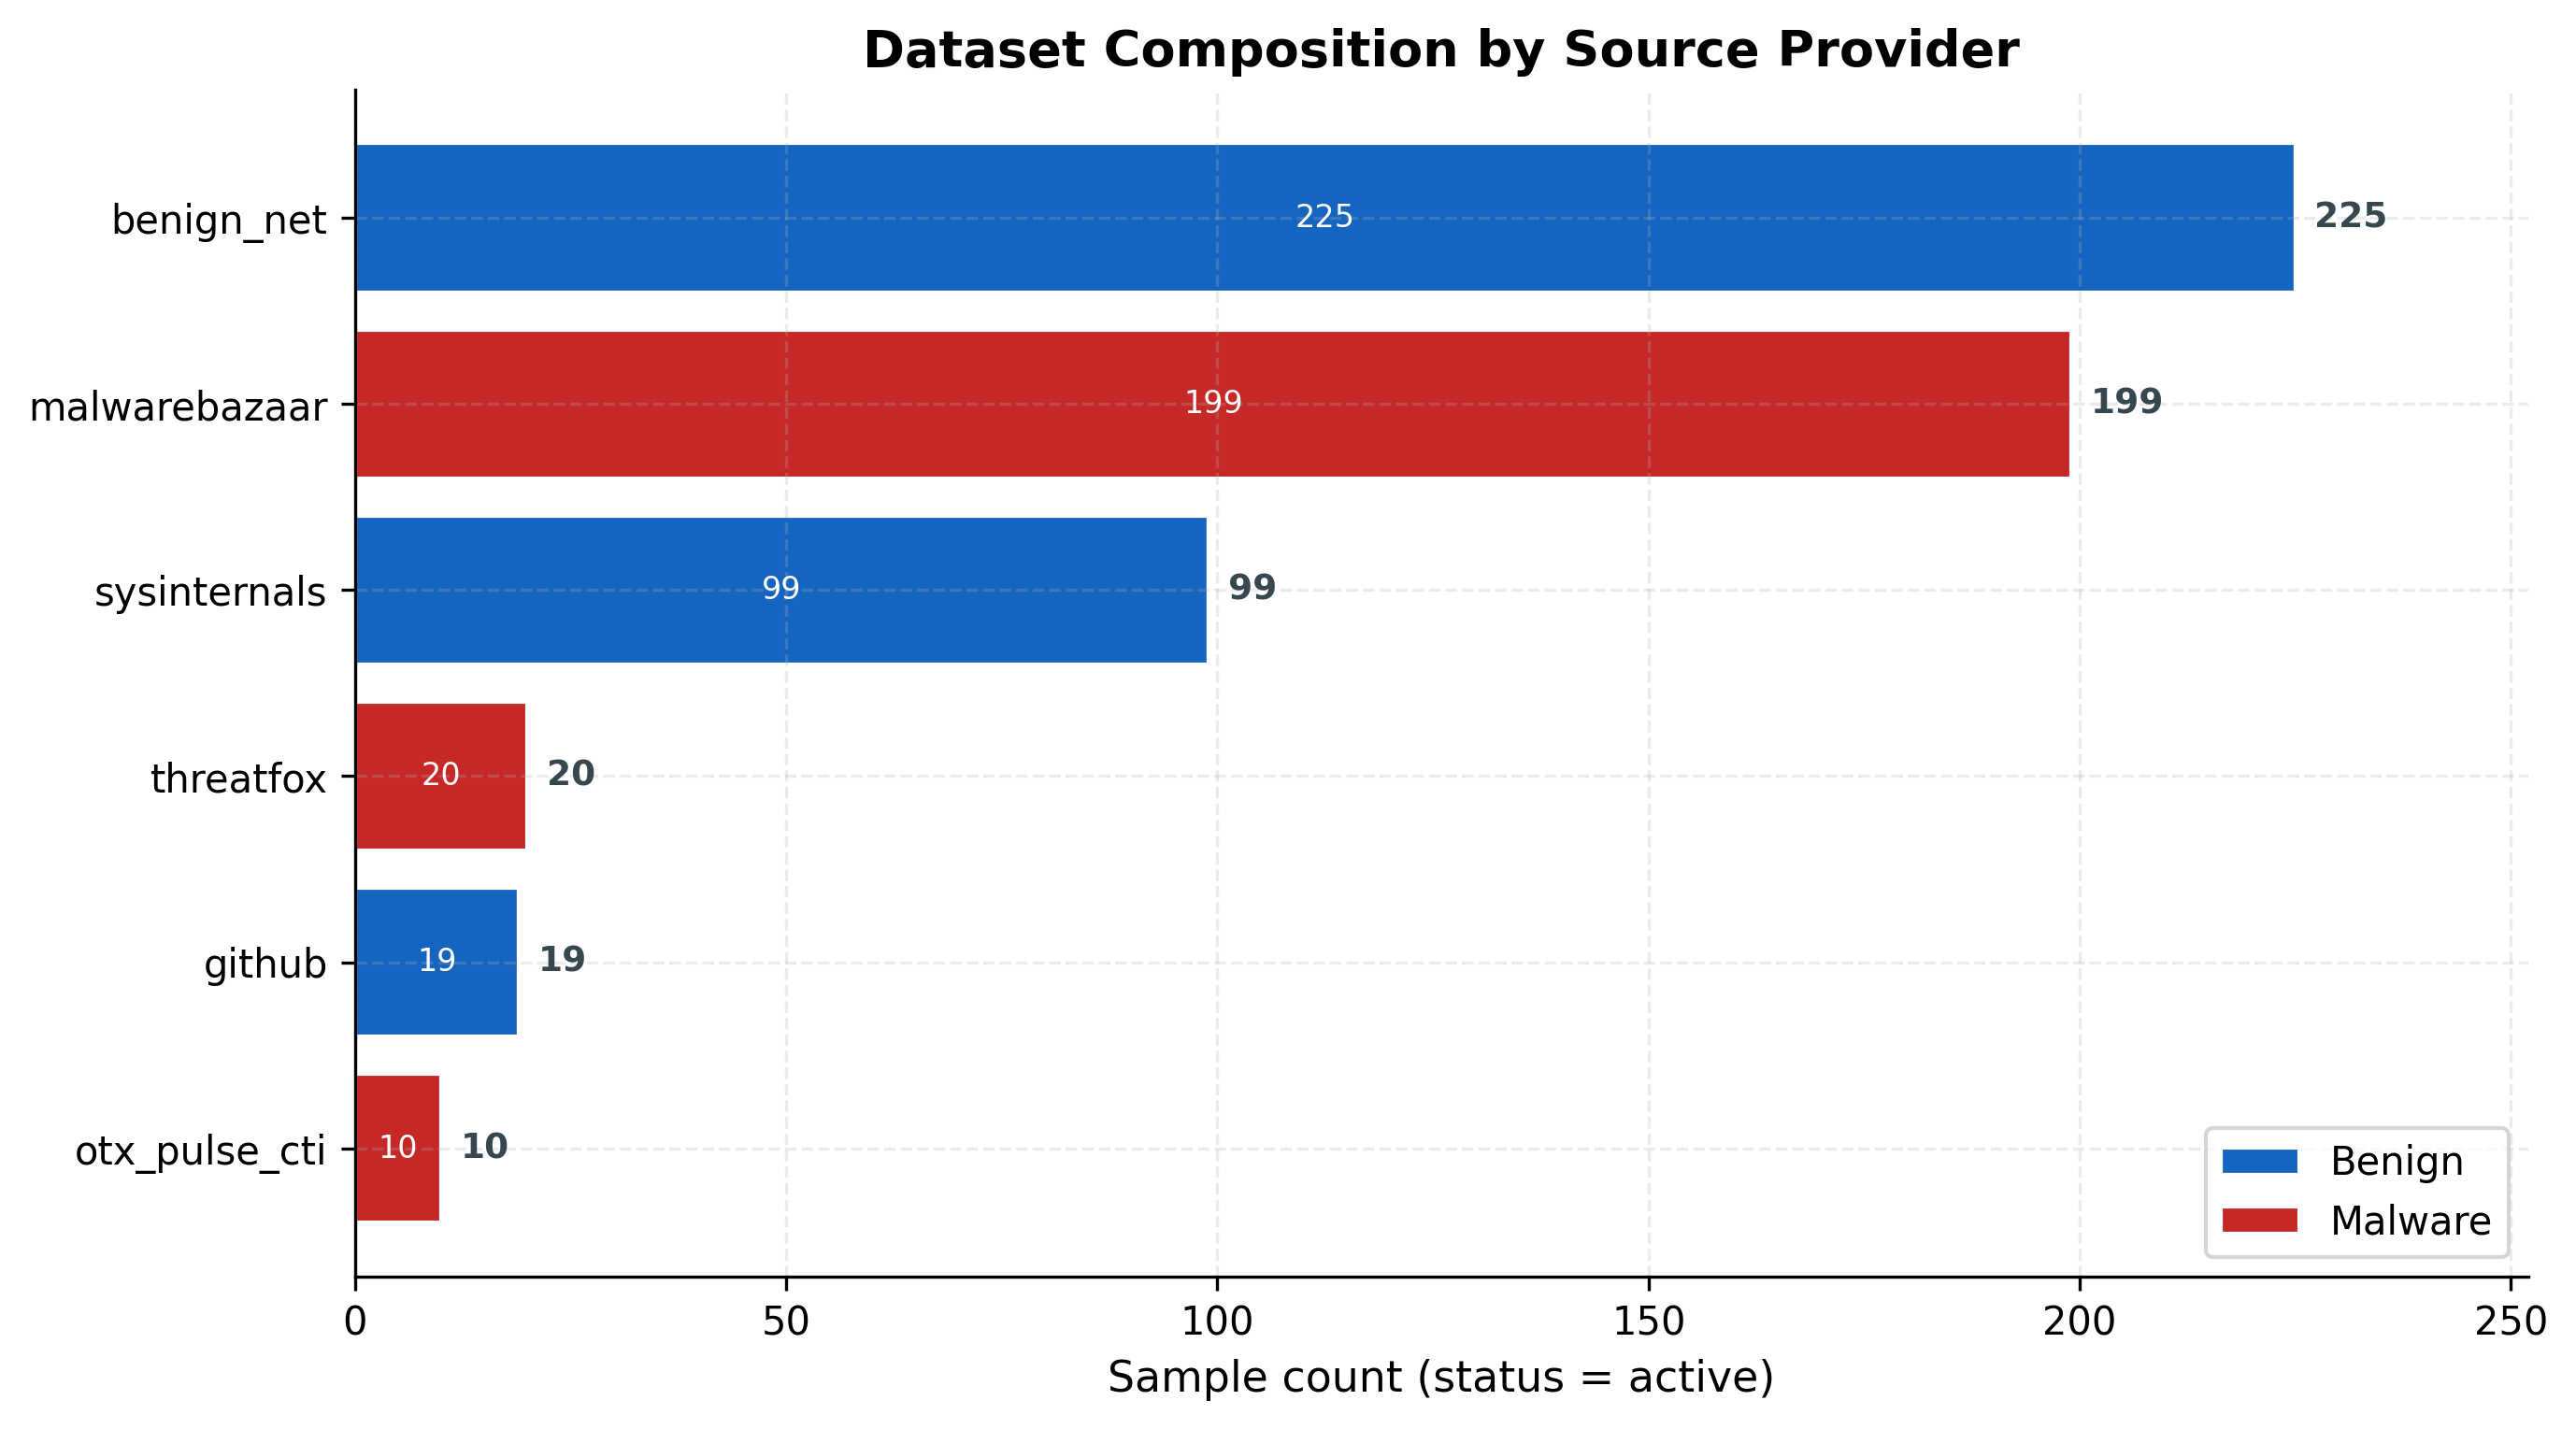
\includegraphics[width=\columnwidth]{figures/data_per_source.png}
\caption{Final active dataset composition by source provider.}
\end{figure}
}{}
\IfFileExists{figures/data_provenance_evolution.png}{%
\begin{figure}[htbp]
\centering
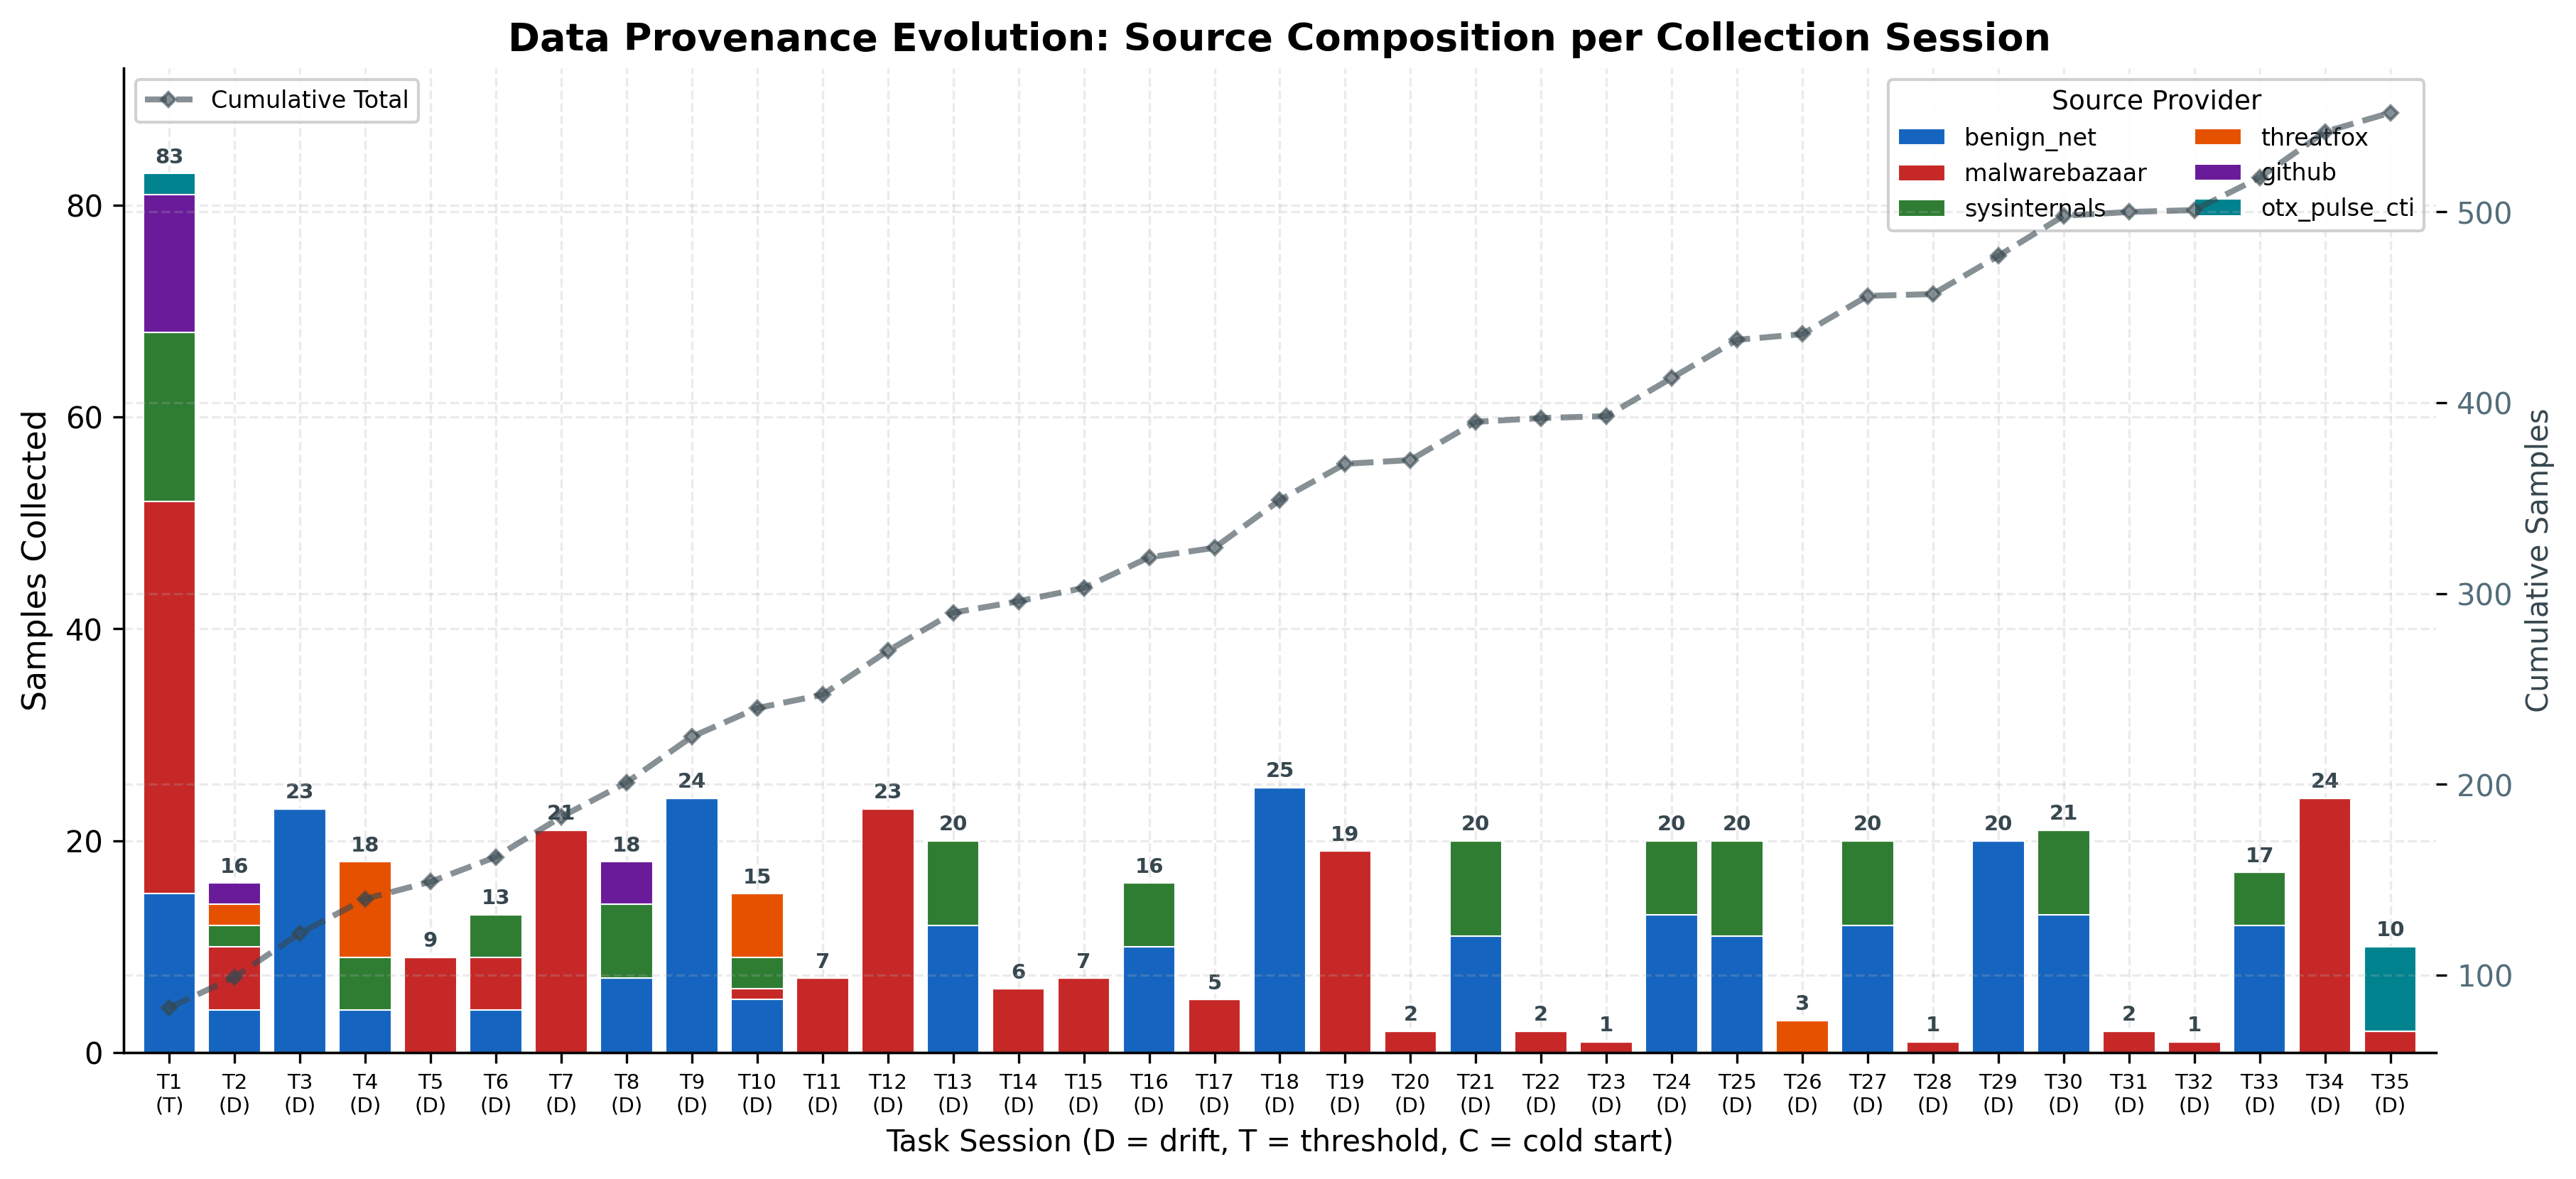
\includegraphics[width=\columnwidth]{figures/data_provenance_evolution.png}
\caption{Source composition over collection sessions.}
\end{figure}
}{}
The final active corpus is drawn from multiple providers rather than a predefined dataset: \texttt{benign\_net} contributes 225 samples, MalwareBazaar 199, Sysinternals 99, ThreatFox 20, GitHub 19, and OTX pulse CTI 10. The provenance timeline shows that collection evolves across sessions instead of staying fixed on one source. Provider outcomes are stored in SQLite, allowing low-yield sources to be ranked lower or cooled down while the agent continues collecting from productive malware and benign providers.

\subsection{Drift and Retraining Impact}
\IfFileExists{figures/drift_per_session.png}{%
\begin{figure}[htbp]
\centering
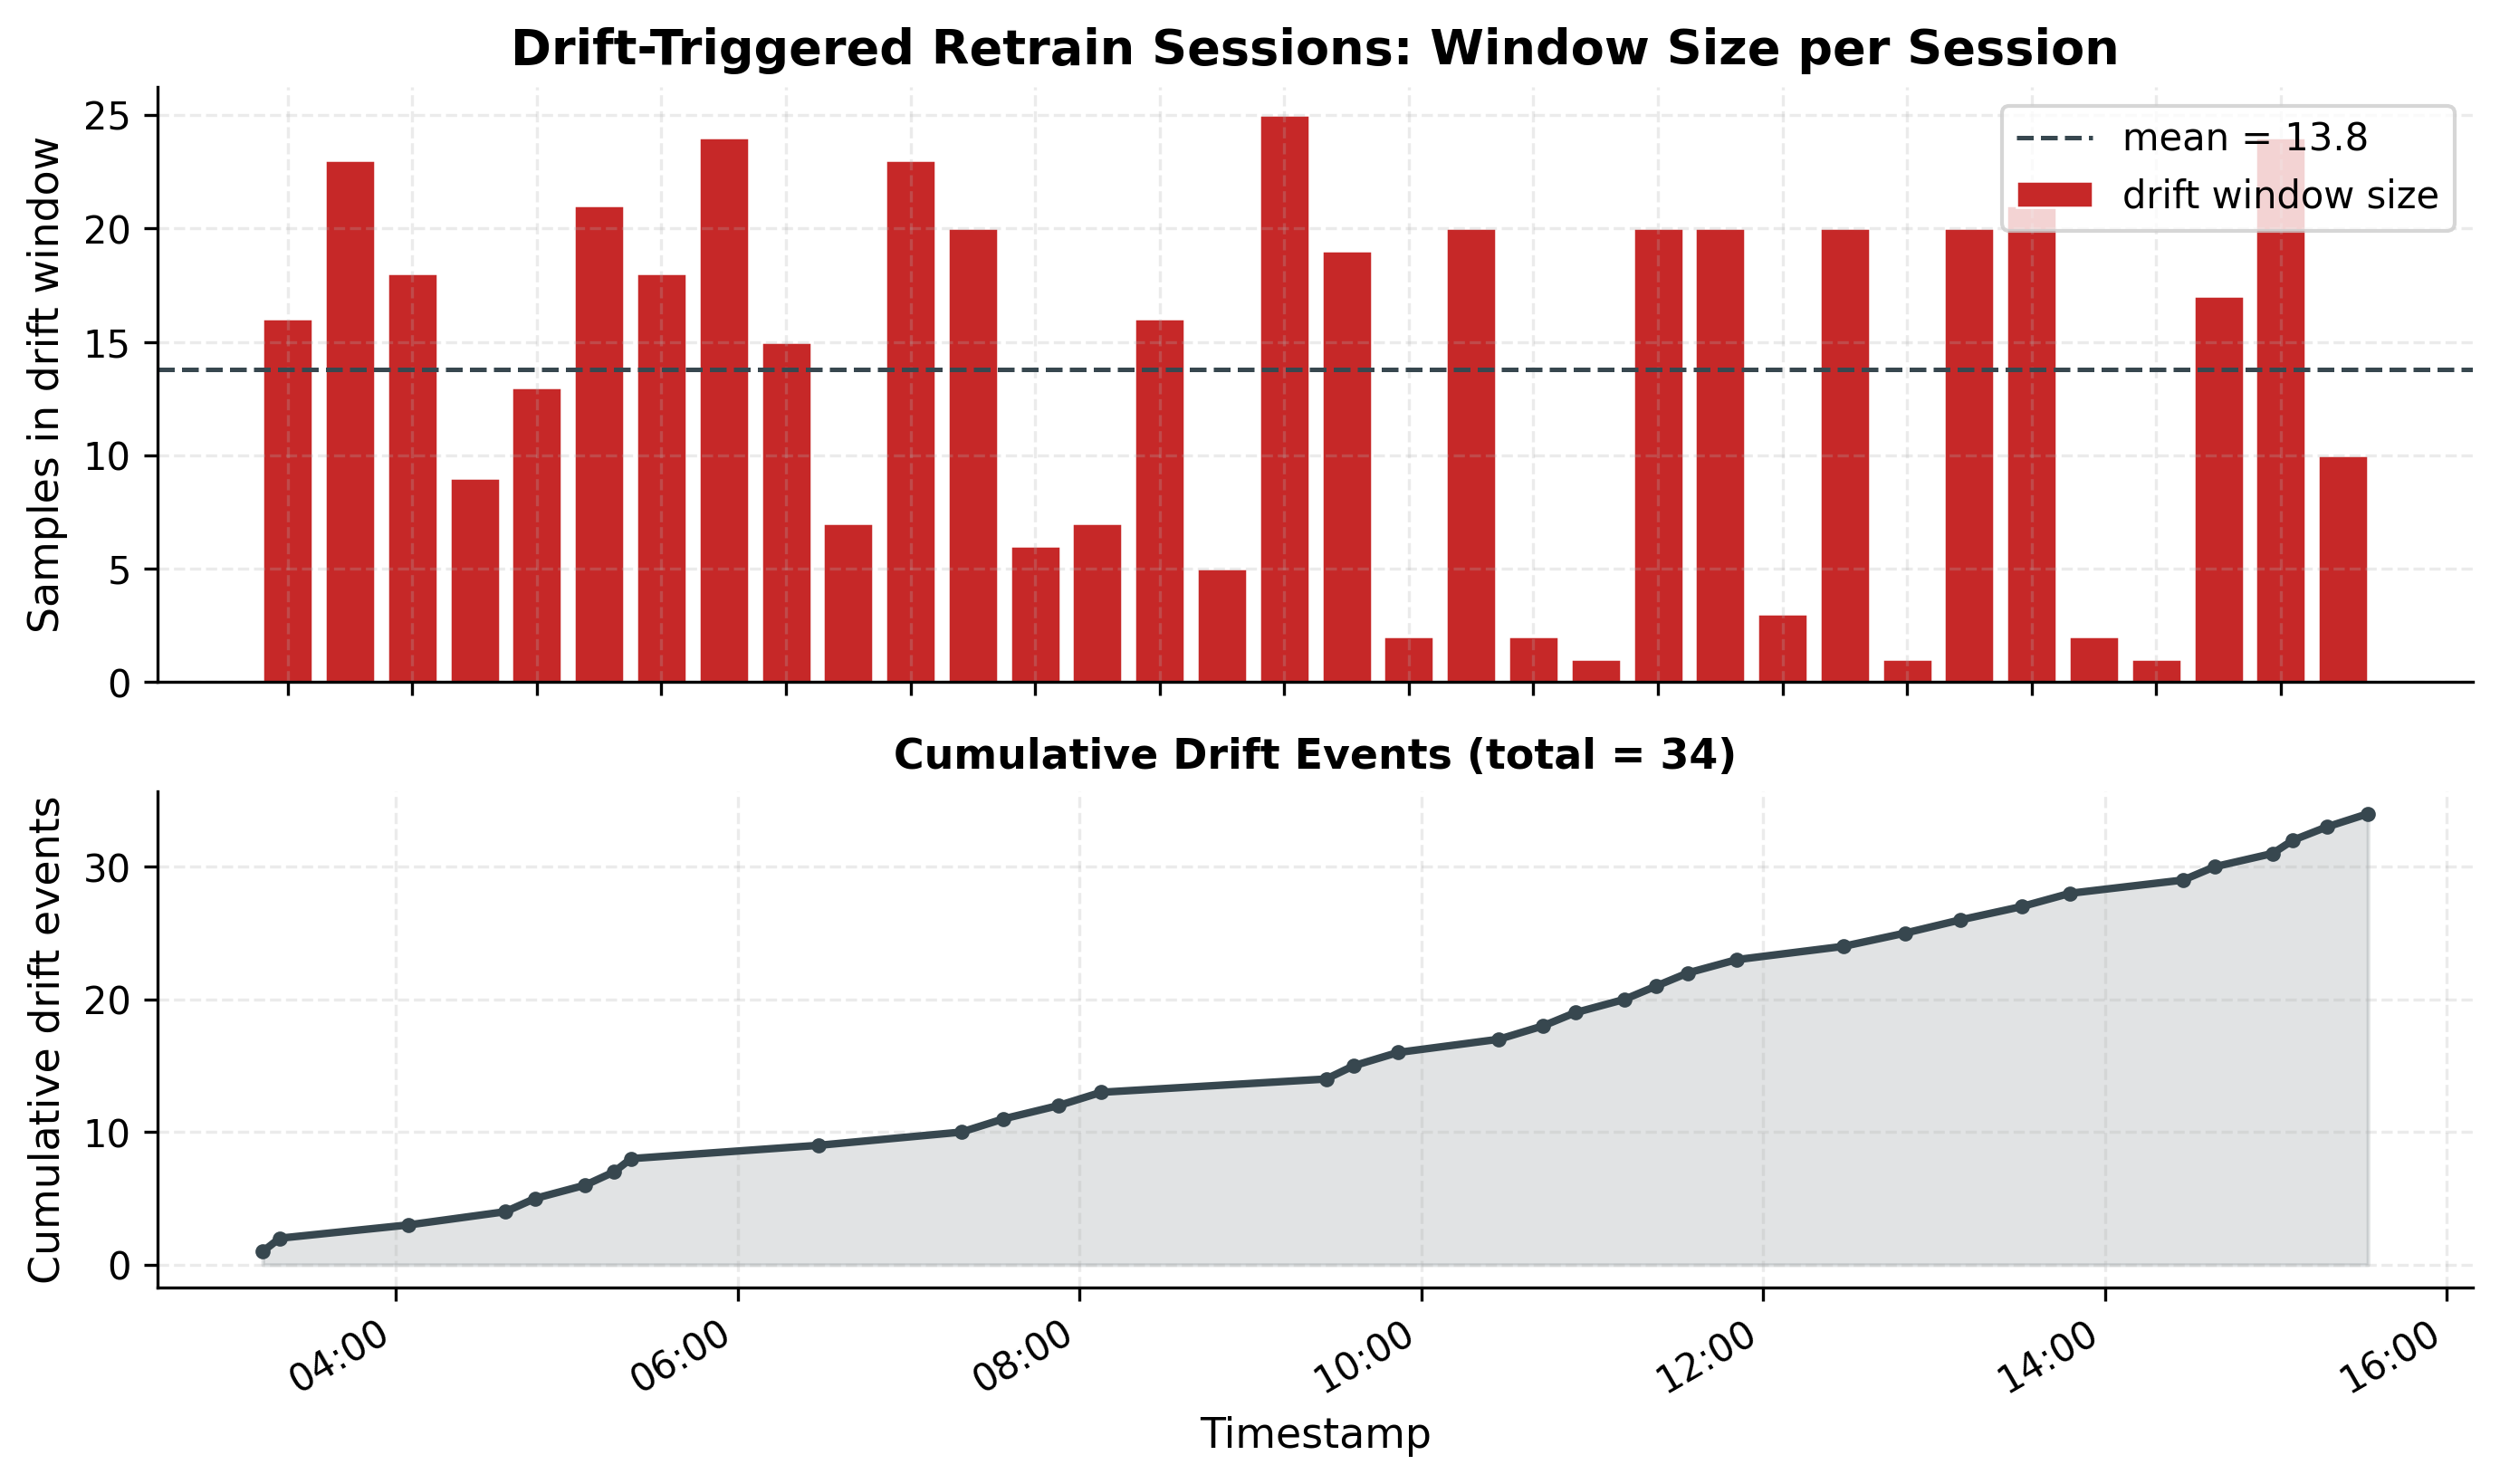
\includegraphics[width=\columnwidth]{figures/drift_per_session.png}
\caption{Drift-triggered retrain sessions and cumulative drift events.}
\end{figure}
}{}
\IfFileExists{figures/drift_retrain_impact.png}{%
\begin{figure}[htbp]
\centering
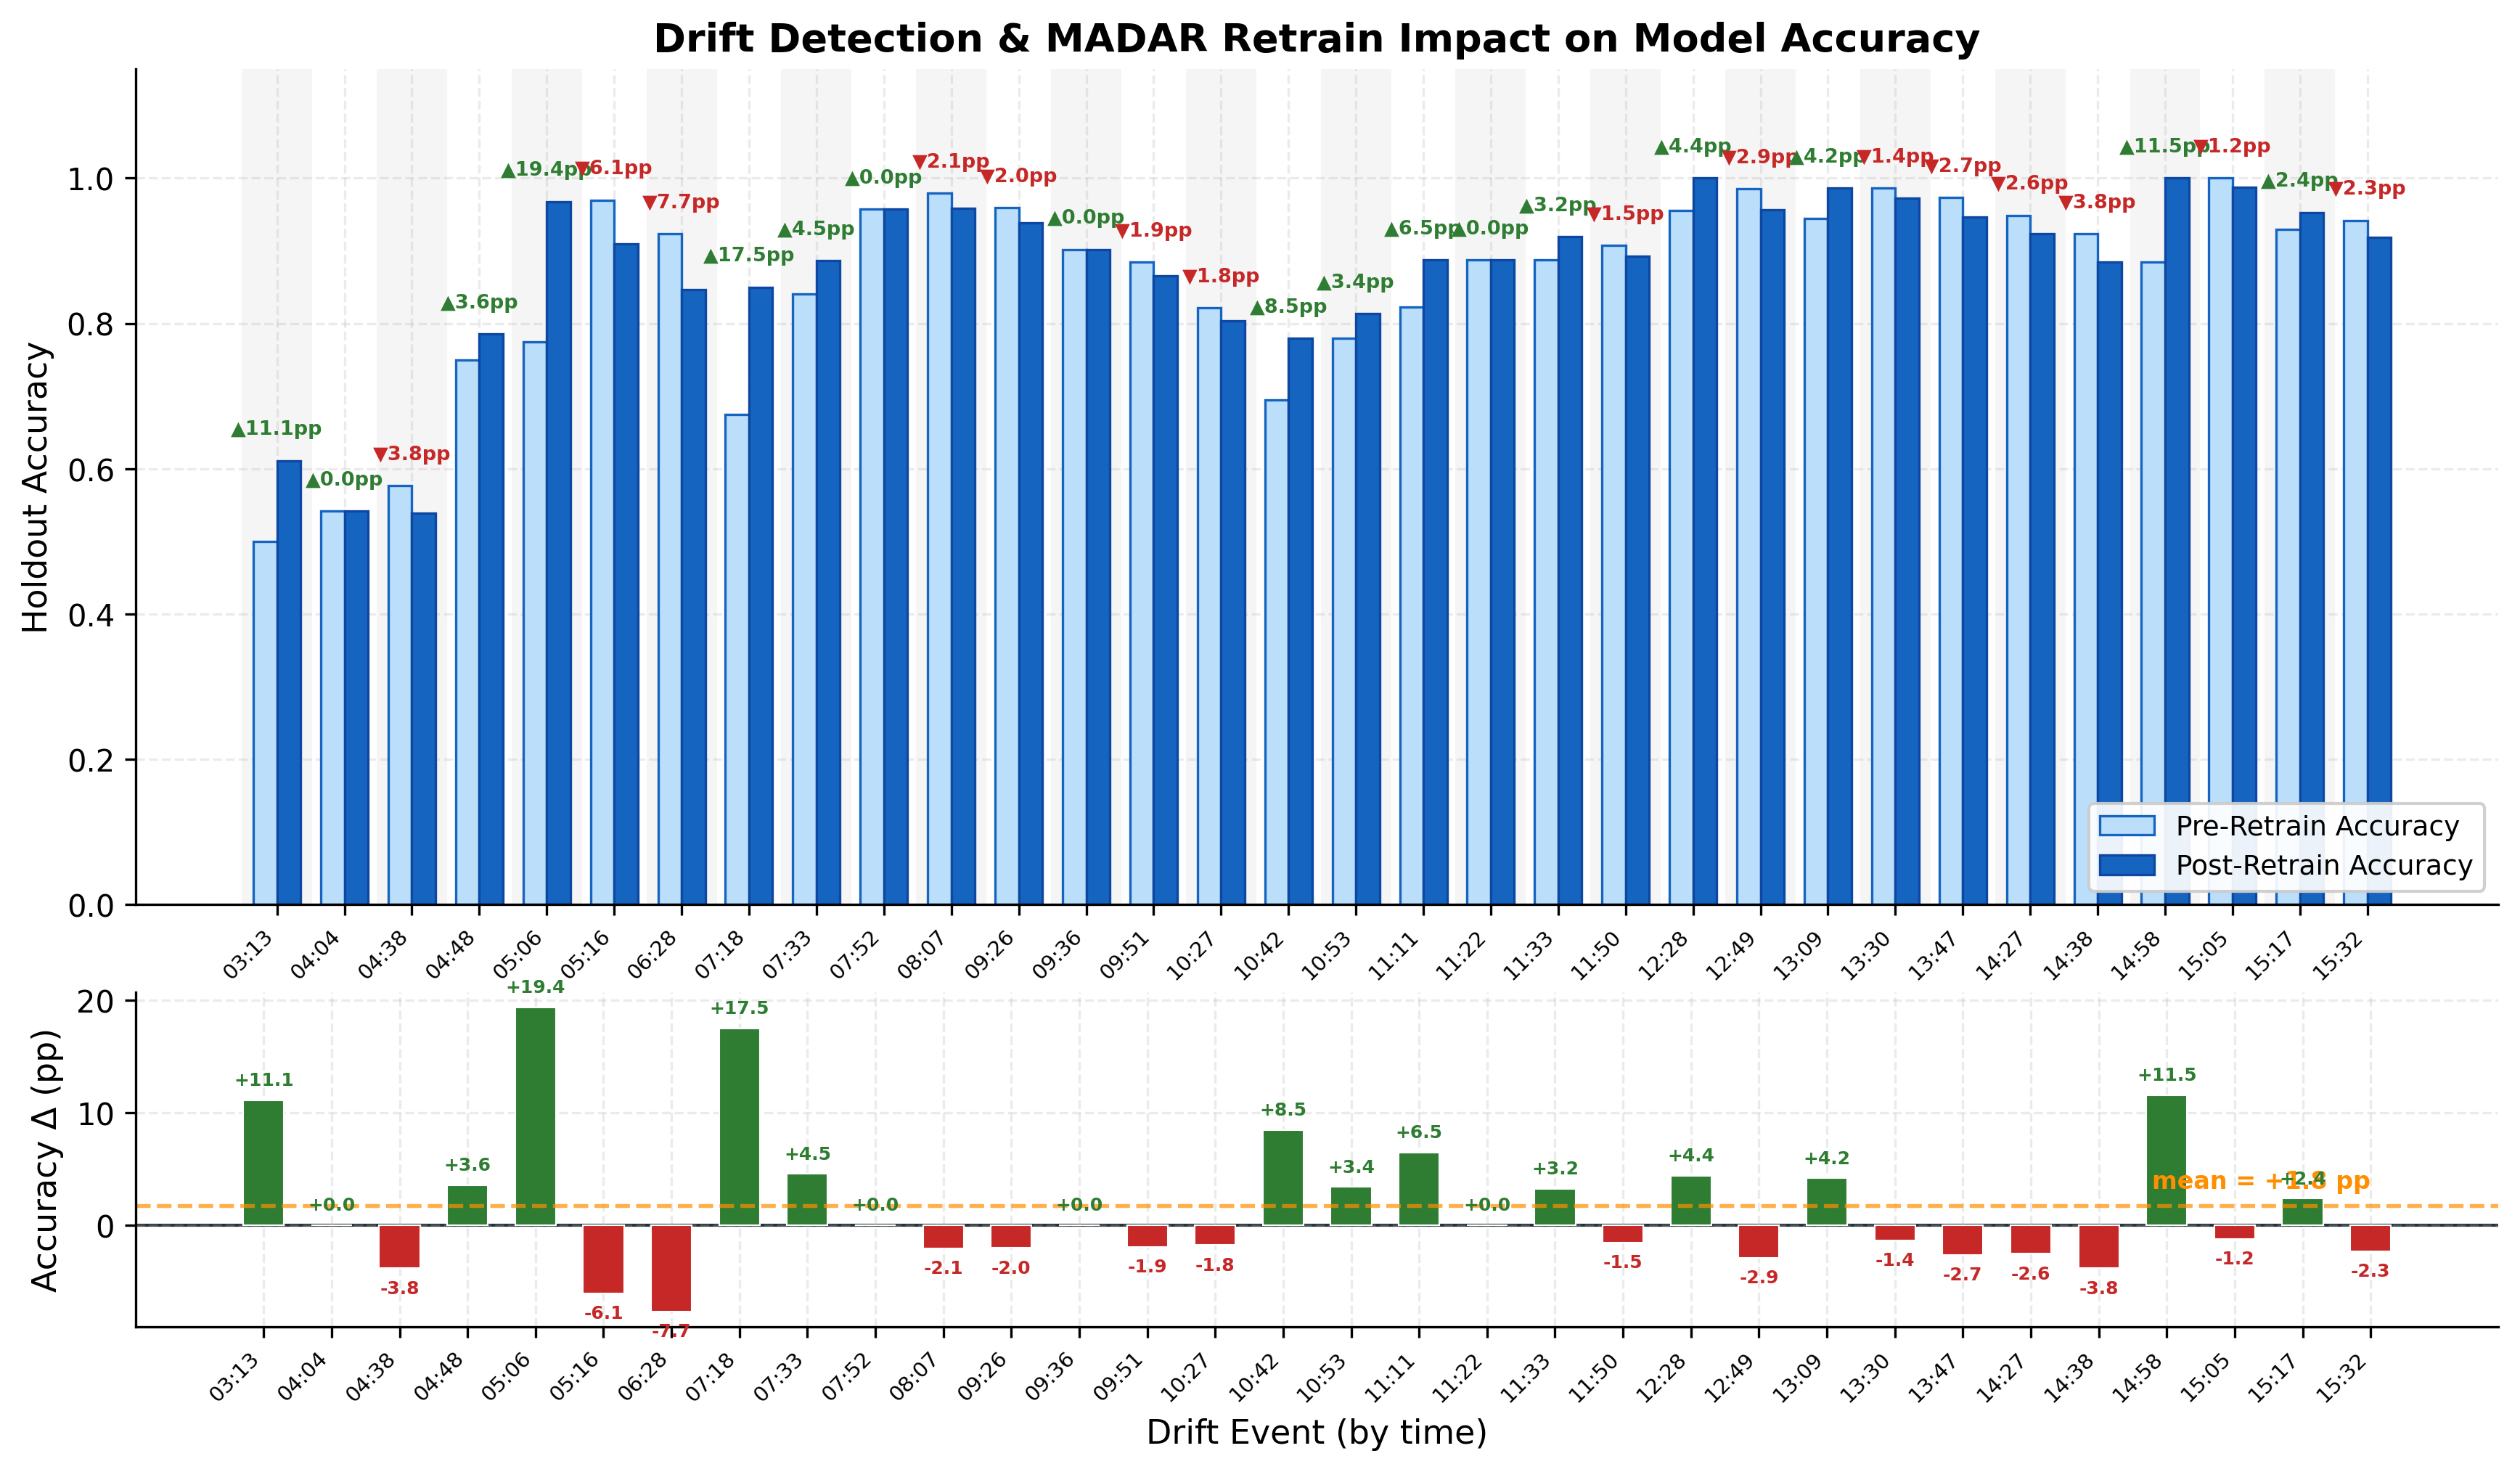
\includegraphics[width=\columnwidth]{figures/drift_retrain_impact.png}
\caption{Pre/post retrain accuracy delta for drift-triggered updates.}
\end{figure}
}{}
The system records 34 drift events, with an average drift window of 13.8 samples. Each drift cycle is documented in \texttt{drift\_log.jsonl}, while model-update comparisons are written to \texttt{model\_update\_log.jsonl}. The pre/post retrain graph shows mixed individual outcomes, including both improvements and regressions, but the mean accuracy delta is positive at approximately $+1.6$ percentage points. This supports the use of MADAR replay as an adaptive recovery mechanism while still exposing cases where retraining does not immediately improve the strict holdout.

\subsection{Model Performance}

To establish the current operational baseline of the pipeline, Figure \ref{fig:confusion_matrix} and Table \ref{tab:model_metrics} present the evaluation metrics for the active LightGBM ml model. The model achieves an exceptional overall accuracy of $98.69\%$ and an Area Under the Curve (AUC) of $0.9989$.

\begin{figure}[htbp]
\centering
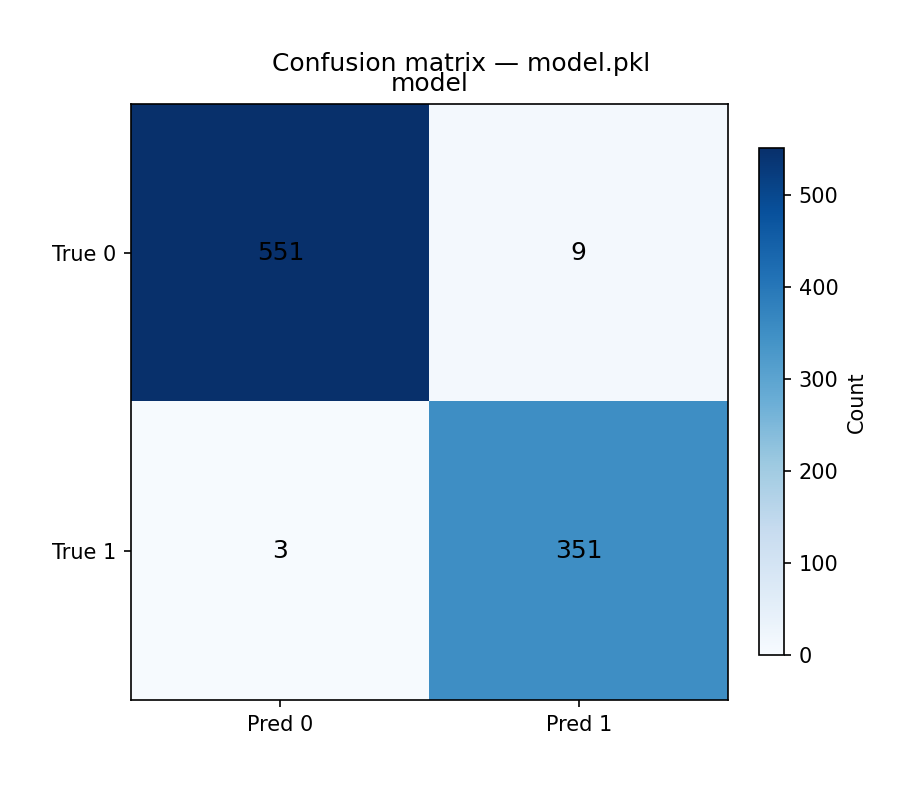
\includegraphics[width=0.85\columnwidth]{figures/confusion_matrices.png}
\caption{Confusion matrix of the active production model.}
\label{fig:confusion_matrix}
\end{figure}

\begin{table}[htbp]
\centering
\caption{Active Production Model Metrics}
\label{tab:model_metrics}
\resizebox{\columnwidth}{!}{%
\begin{tabular}{@{}ccccc@{}}
\toprule
\textbf{Accuracy} & \textbf{Precision} & \textbf{Recall (TPR)} & \textbf{FPR} & \textbf{AUC} \\
\midrule
98.69\% & 97.50\% & 99.15\% & 1.61\% & 0.9989 \\
\bottomrule
\end{tabular}%
}
\end{table}

The dynamic threshold calibration successfully bounds the False Positive Rate to $1.61\%$ while maintaining a highly aggressive True Positive Rate (Recall) of $99.15\%$. As visualized in the confusion matrix, this strict recall-favored tuning results in only 3 False Negatives out of the testing sample, ensuring that novel malware variants do not easily bypass the static feature filters during the steady state.

*The evaluation have been tested on data set of 914.
\section{Critical Analysis and Limitations}

\begin{itemize}
  \item The agent successfully avoids a predefined dataset by collecting from live providers, but this makes throughput dependent on MalwareBazaar, OTX, ThreatFox, GitHub, and benign repositories. Provider cooldowns reduce wasted attempts, but rate limits and downtime still affect collection.

  \item The results show that MADAR replay usually helps recovery, but not every retraining event improves the strict holdout. This is why the system logs before/after deltas instead of assuming each update is beneficial.

  \item Drift detection is intentionally disabled during bootstrap, so early sparse labels can bypass drift validation until the initial corpus and model are ready.

  \item TESSERACT evaluation is more realistic than random splits, but it must skip windows where the chronological holdout is too small or single-class.

  \item Static PE features are safe and fast, but packed or obfuscated binaries can hide imports, strings, and opcode patterns, increasing false-negative risk.

  \item Ollama improves CTI filtering and drift explanations, but remains best-effort. Deterministic validation and fallback logic are still required for safety.


\end{itemize}

\section{Conclusion}
AMD-Agent demonstrates a Docker-first autonomous malware detection agent that builds its dataset from live sources rather than a predefined corpus. The system combines LangGraph orchestration, safe PE acquisition, static feature extraction, LLM-assisted CTI filtering, provider reliability tracking, ADWIN drift detection, MADAR replay retraining, and strict chronological before/after evaluation. The results show that the agent can continue collecting data, detect drift, and usually recover performance after retraining, while still exposing regressions through model-update logs. Future work includes expanding LangGraph subgraphs for multi-agent validation, improving source discovery, and integrating reinforcement learning for source selection.

\bibliographystyle{IEEEtran}
\bibliography{references}

\end{document}